At the end of this worksheet you should be able to  
\begin{itemize}
	\item to discuss the relationships between the quantities of work, energy, displacement, velocity.
	\item differentiate between a conservative force and a non-conservative force.
	\item apply the work energy theorem to solve interesting problems that would be hard to use Newton's Laws.
	\item discuss the principle of conservation of energy and explain when it is useful.
\end{itemize}


\begin{enumerate}
\setlength\itemsep{1 in}

\item
\emph{Work} is defined as a transfer of \emph{energy}. This transfer occurs by one object exerting a force on another object \emph{over some displacement}. But the relative directions of these two vector quantities (force and displacement) matters. Summarize the work done in 5 different cases that are represented below by drawing the object and the vectors representing force $\vec{F}$ and displacement $\Delta \vec{x}$. In each case I have provided a simple example to illustrate what I mean. You provide another one.
\begin{itemize}
	\setlength\itemsep{1 in}
	\item The force and displacement point in exactly the same direction. (I push a box across a level floor with  \SI{100}{\newton} a distance of \SI{10}{\meter}).
    \item The force and displacement point in different directions, but the angle between them is less than \ang{90}. (I pull a box across a level floor with a string, directing \SI{100}{\newton} at an angle of \ang{20} with respect to the floor.)
    \item The force and the displacement are exactly perpendicular to each other. (A \SI{10}{kg} box is sliding across a friction-less surface, and the normal force is acting on the box.)
    \item The force and displacement point in different directions and the angle between them is greater than \ang{90}. (I bring a sliding box to a stop by exerting a \SI{100}{\newton} force on it at and angle of \ang{30} with respect to the horizontal.)
    \item The force and displacement point in exactly opposite directions. (I bring a sliding box to a stop by exerting a \SI{100}{\newton} force over a distance of \SI{10}{\meter}.)
\end{itemize}

\item
What amount of work is done by a person to lift a \SI{100}{kg} object a distance of \SI{1}{meter} high? What amount of work is done by the force of gravity? If the person dropped the box what amount of work would the force of gravity do on the box as it fell? What velocity would it achieve before it hit the ground?

\item What amount of work is required to push a \SI{100}{kg} object up a friction-less inclined plane of that is \SI{10}{\meter} long that's end it \SI{1}{meter} high? How does this compare to the work done to lift it? Show that this can be used to derive the formula $\frac{F_{\mathrm{push}}}{\mathit{weight}}=\frac{\mathit{height}}{l_{\mathrm{plane}}}$.\bigskip

\item An object has some initial velocity at the bottom of a friction-less ramp and it begins to slide up the ramp. The force of gravity does negative work here and the object slows down to stop. The ramp has an incline angle of \ang{20} with respect to the horizontal. Calculate the work done by the force of gravity and see that it is a negative value in three ways:
\begin{itemize}
	\setlength\itemsep{1 in}
	\item What is the angle between the displacement and the force of gravity? Use this angle and the definition of work to calculate the work.
	\item What is another angle between the displacement and the force of gravity? Now use this angle and the definition of work to calculate the work.
	\item What is the \emph{component} of the force of gravity that is in the direction of the displacement? Are these vectors in the same direction or opposite directions? What is the work done using component and the displacement? 
\end{itemize}

\item 
\emph{Kinetic energy} is the energy of an object that has velocity. In order to calculate it, use $K = \frac{1}{2}mv^2$. Calculate the kinetic energy of a \SI{10}{kg} object that has a velocity of \SI{10}{m/s}. If you do some work to \emph{double} the velocity of the object, what is the new kinetic energy? What is the ratio of the kinetic energy final to the initial kinetic energy? What is the \emph{change} in kinetic energy? How much \emph{work} would be required to cause this change in kinetic energy? If this was done by a force pointed in the direction of the objects motion acting over a distance of 10 meters, what is the magnitude of the force?\hugeskip

\item I push an object at constant velocity of \SI{1}{m/s} over a friction-full surface. I exert a force of \SI{100}{\newton} and do this over a distance of \SI{10}{\meter}. What work have I done? What work has the force of friction done? What is the net work done? What is the kinetic energy initially? Does the kinetic energy change? What power am I providing?
\bigskip

\item 
I pull a \SI{10}{kg} object with a rope at an angle of \ang{20} to a horizontal friction-full surface. I use a force of \SI{100}{\newton} on the rope, and the coefficient of kinetic friction is $\mu=0.1$. I start at rest and exert this force over a distance of \SI{100}{\meter}. 
\begin{itemize}
	\setlength\itemsep{1 in}
	\item What work do I do?
	\item What work does the force of friction do?
	\item What work does the normal force do?
	\item What work does the force of gravity do?
	\item Using these works, what is the net work?
	\item What is the change in kinetic energy?
	\item What is the final velocity?
	\item What is the net force?
	\item Using the net force, what is the net work?
\end{itemize}

\item What forces are conservative forces and what are not conservative forces?

\item 
When a \SI{10}{kg} object is \SI{10}{\meter} high, what is its potential energy? If it begins it to fall, what is its potential energy after it falls \SI{1}{\meter}? How much has its kinetic energy changed?

\item 
An object falls from a height of \SI{100}{\meter} then how fast is it going when it hits the ground? Solve this using kinematics an then again using conservation of energy? \bigskip

\item 
A roller coaster starts from rest at the top of a hill and rolls down its course. Find its kinetic and potential energy at each position marked.\\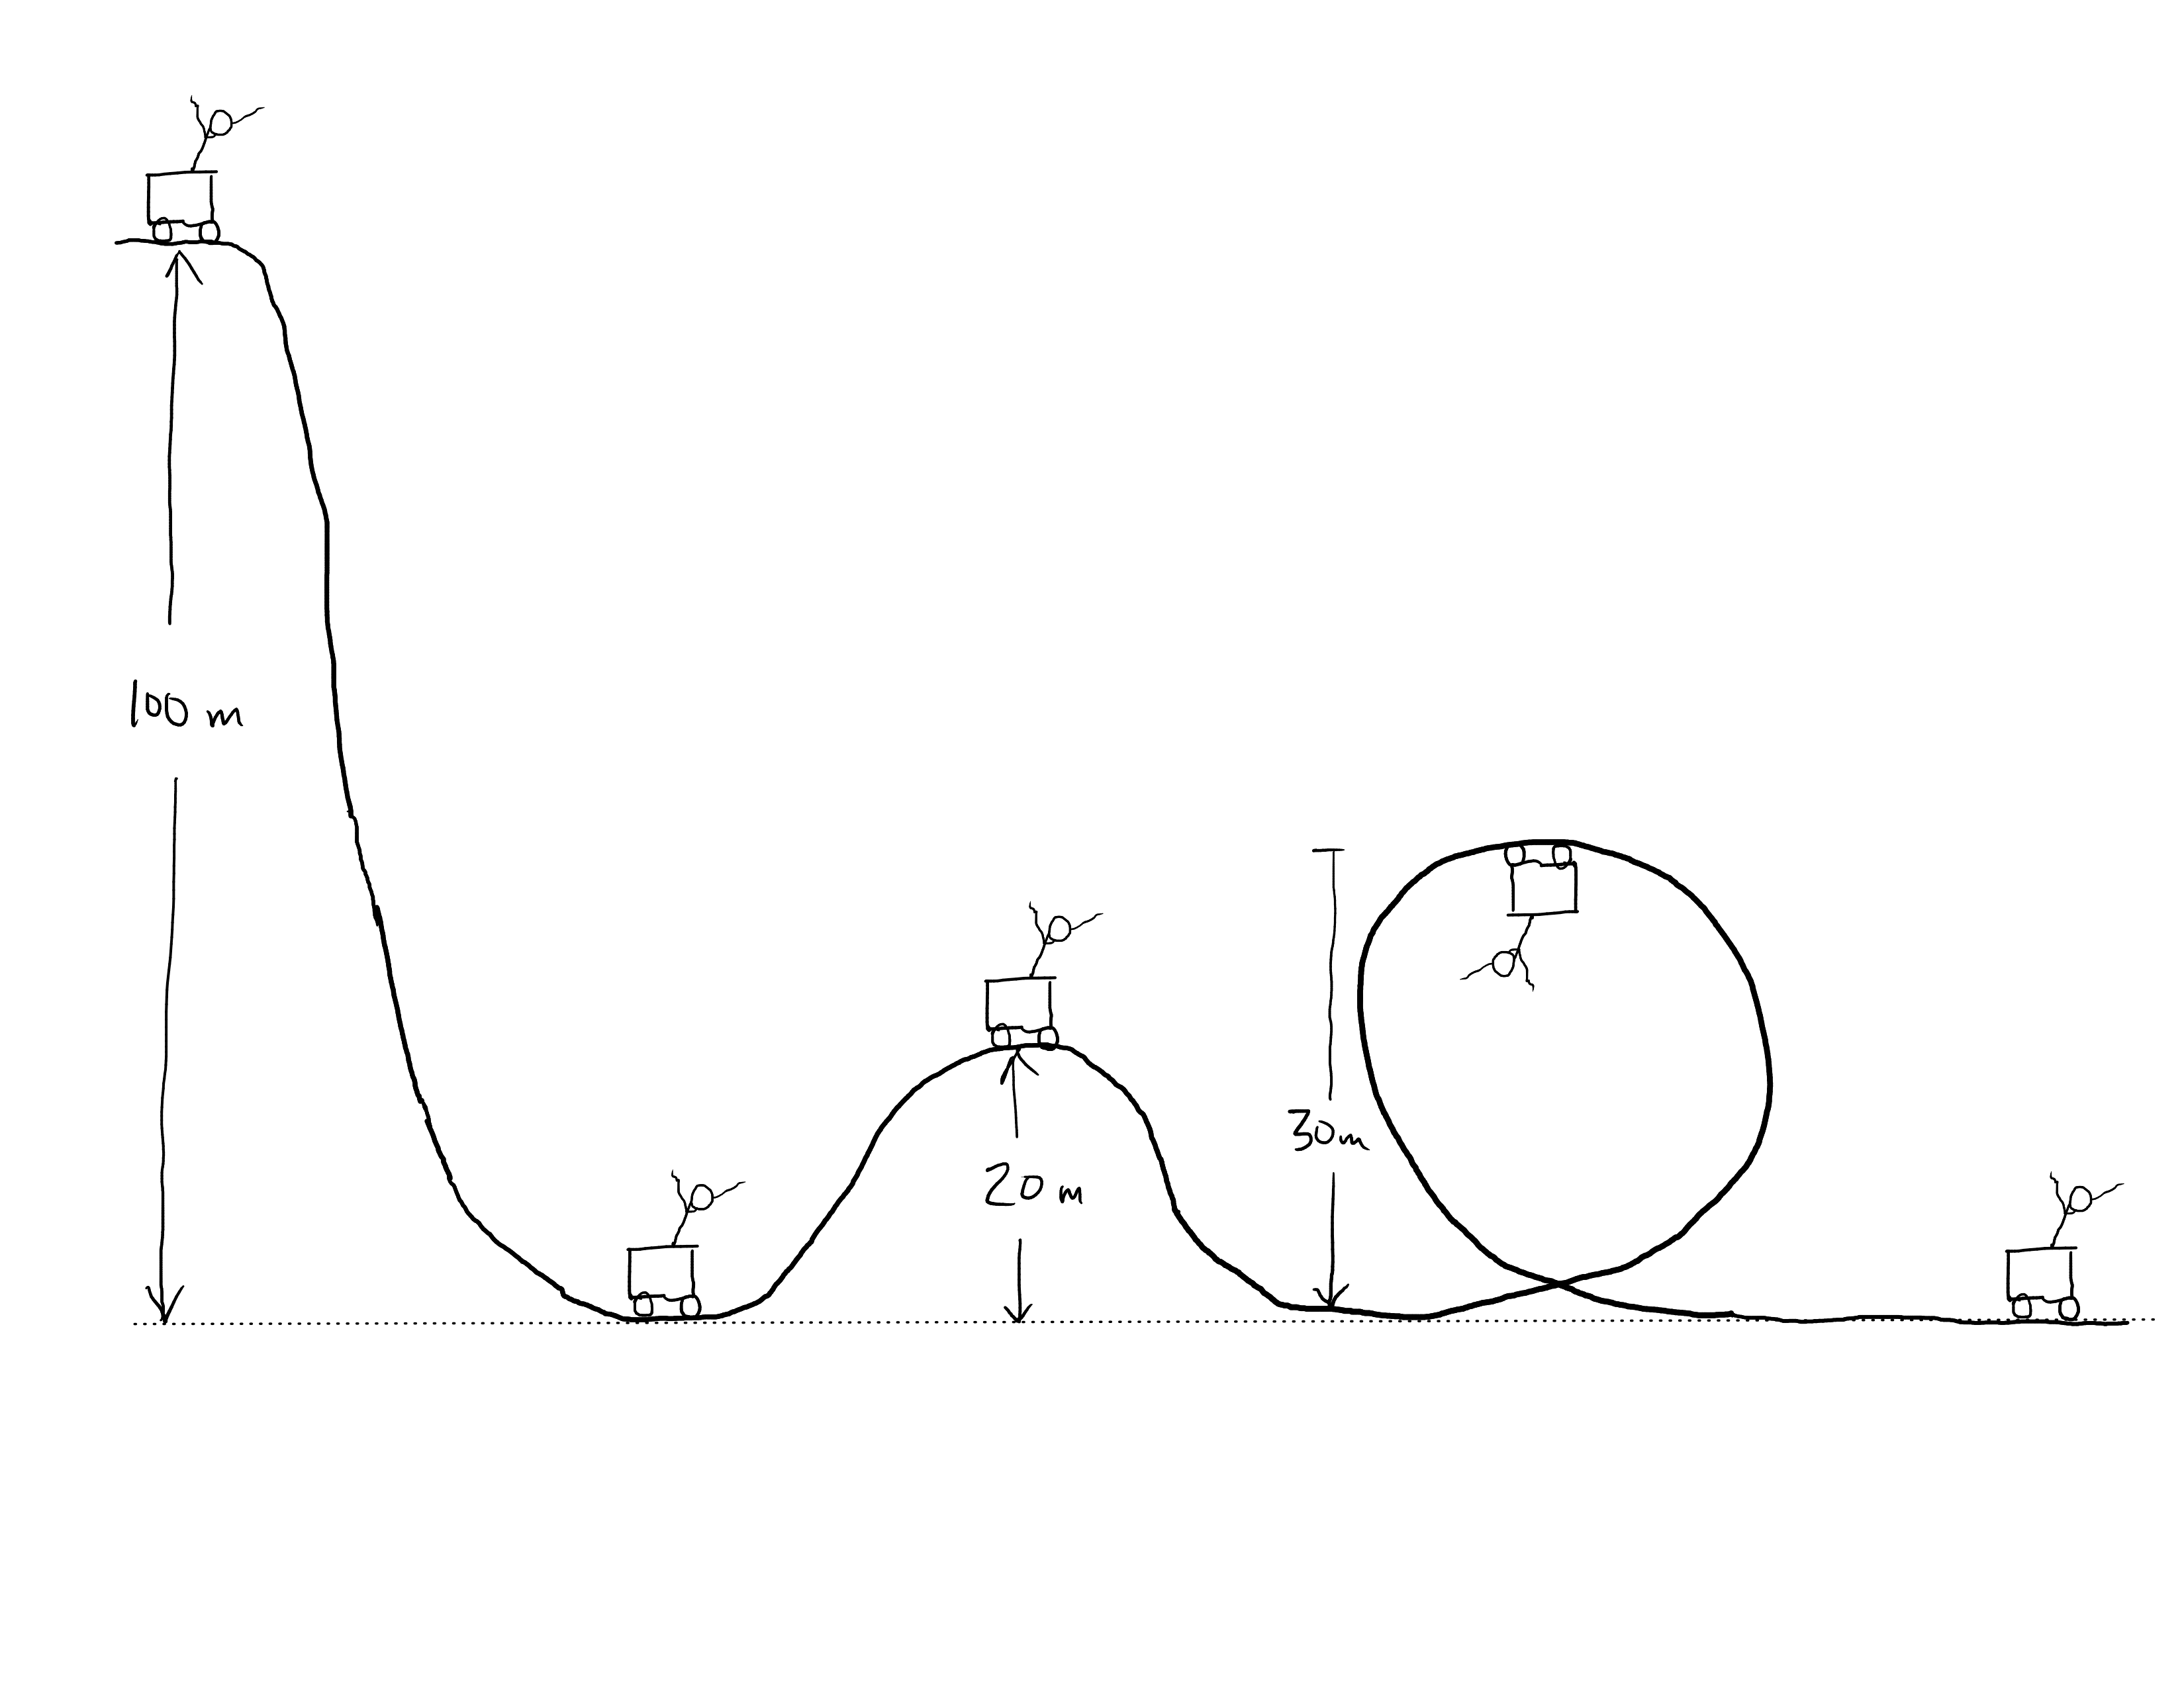
\includegraphics[scale=0.1]{week7-roller-coaster.png}

\item 
A \SI{10}{kg} box slides down a friction-full inclined plane ($\mu=0.1, \theta=\ang{30}$). The height of the plane is \SI{1}{\meter} above the horizontal. What is the speed of the box at the bottom of the plane? How does this compare to if there were no friction? How much work has been done by the force of friction?\hugeskip

\item 
Here is an example of a problem that would be much more difficult to do with Newton's Laws. Take the same inclined plane as the problem above, but make \emph{most} of the plane friction-less and only a \SI{10}{cm} portion in the middle of the plane have friction $\mu=0.1$. Now what is the speed at the bottom of the plane? Think about how you would have solved this using Newton's Laws and kinematics. \bigskip

\item 
The maximum speed of a child on a swing is \SI{5}{m/s}. At this point the child is \SI{1}{\meter} above the ground. What is the maximum height of the child above the ground? Do this two ways, once with $U_g = 0$ at the ground, and once again with $U_g=0$ at the bottom of the swing's path.\bigskip

\item 
A \SI{100}{\kilogram} cyclist (and bike) has at constant speed of \SI{10}{m/s} up an incline of 5\% (vertical height/horizontal distance as a percent). What power output does the rider need to provide to do this? 

\item 
A pendulum swings from some maximum height where its velocity is zero to a minimum where is velocity is a maximum and then back up to a maximum height. If the maximum height is 0.1 meters above the minimum height, then what is the speed of the pendulum at the bottom of its swing?

\item 
For a pendulum, it is hard to measure its maximum height, but it is easy to measure its length and to measure its angle from the vertical. If the maximum angle from the vertical of a \SI{1}{\meter} long pendulum is \ang{20} then how high is this above the horizontal? (\emph{Hint: draw a line from the end of the pendulum when it is at its maximum height perpendicularly to the line when it is at is minimum height.})\\ 

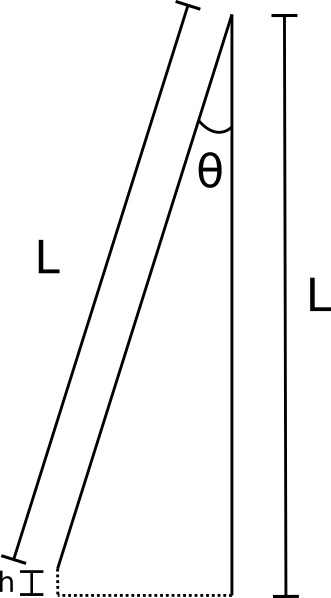
\includegraphics[]{pendulum-h-l-theta.png} 

\item 
A horse pulls a \SI{250}{kg} cart a distance of \SI{1.5}{km}. The frictional force on the cart is a constant \SI{250}{\newton}. The horse eats oats in the morning to prepare for this trip. Each gram of oats provides \SI{10}{\kilo\joule} of energy, but only 10\% of this energy can go into work pulling the cart. How many grams of oats must the horse eat?

\item
I want to try a weight loss program that involves repeatedly lifting a \SI{50}{kg} barbell from the ground to over my head at a height of \SI{2}{\meter}. I can do this about 5 times per minute. How long will it take me to burn \SI{0.5}{kg} of fat? ``Burning'' fat means I have used it to supply energy to do work. Each gram of fat has roughly \SI{39}{\kilo\joule} of energy to the body, but the muscles can only use 10\% of this to do work. 

\item What is the minimum height $h$ that a roller coaster needs to start at rest in order to do a loop-the-loop of radius $r$ and not lose contact with the track?


\item 
If you are doing a rope swing and then at the lowest point in the swing you let go and drop into a lake below, how far from the edge of the cliff do you land in the water. See the diagram below for the relevant parameters.

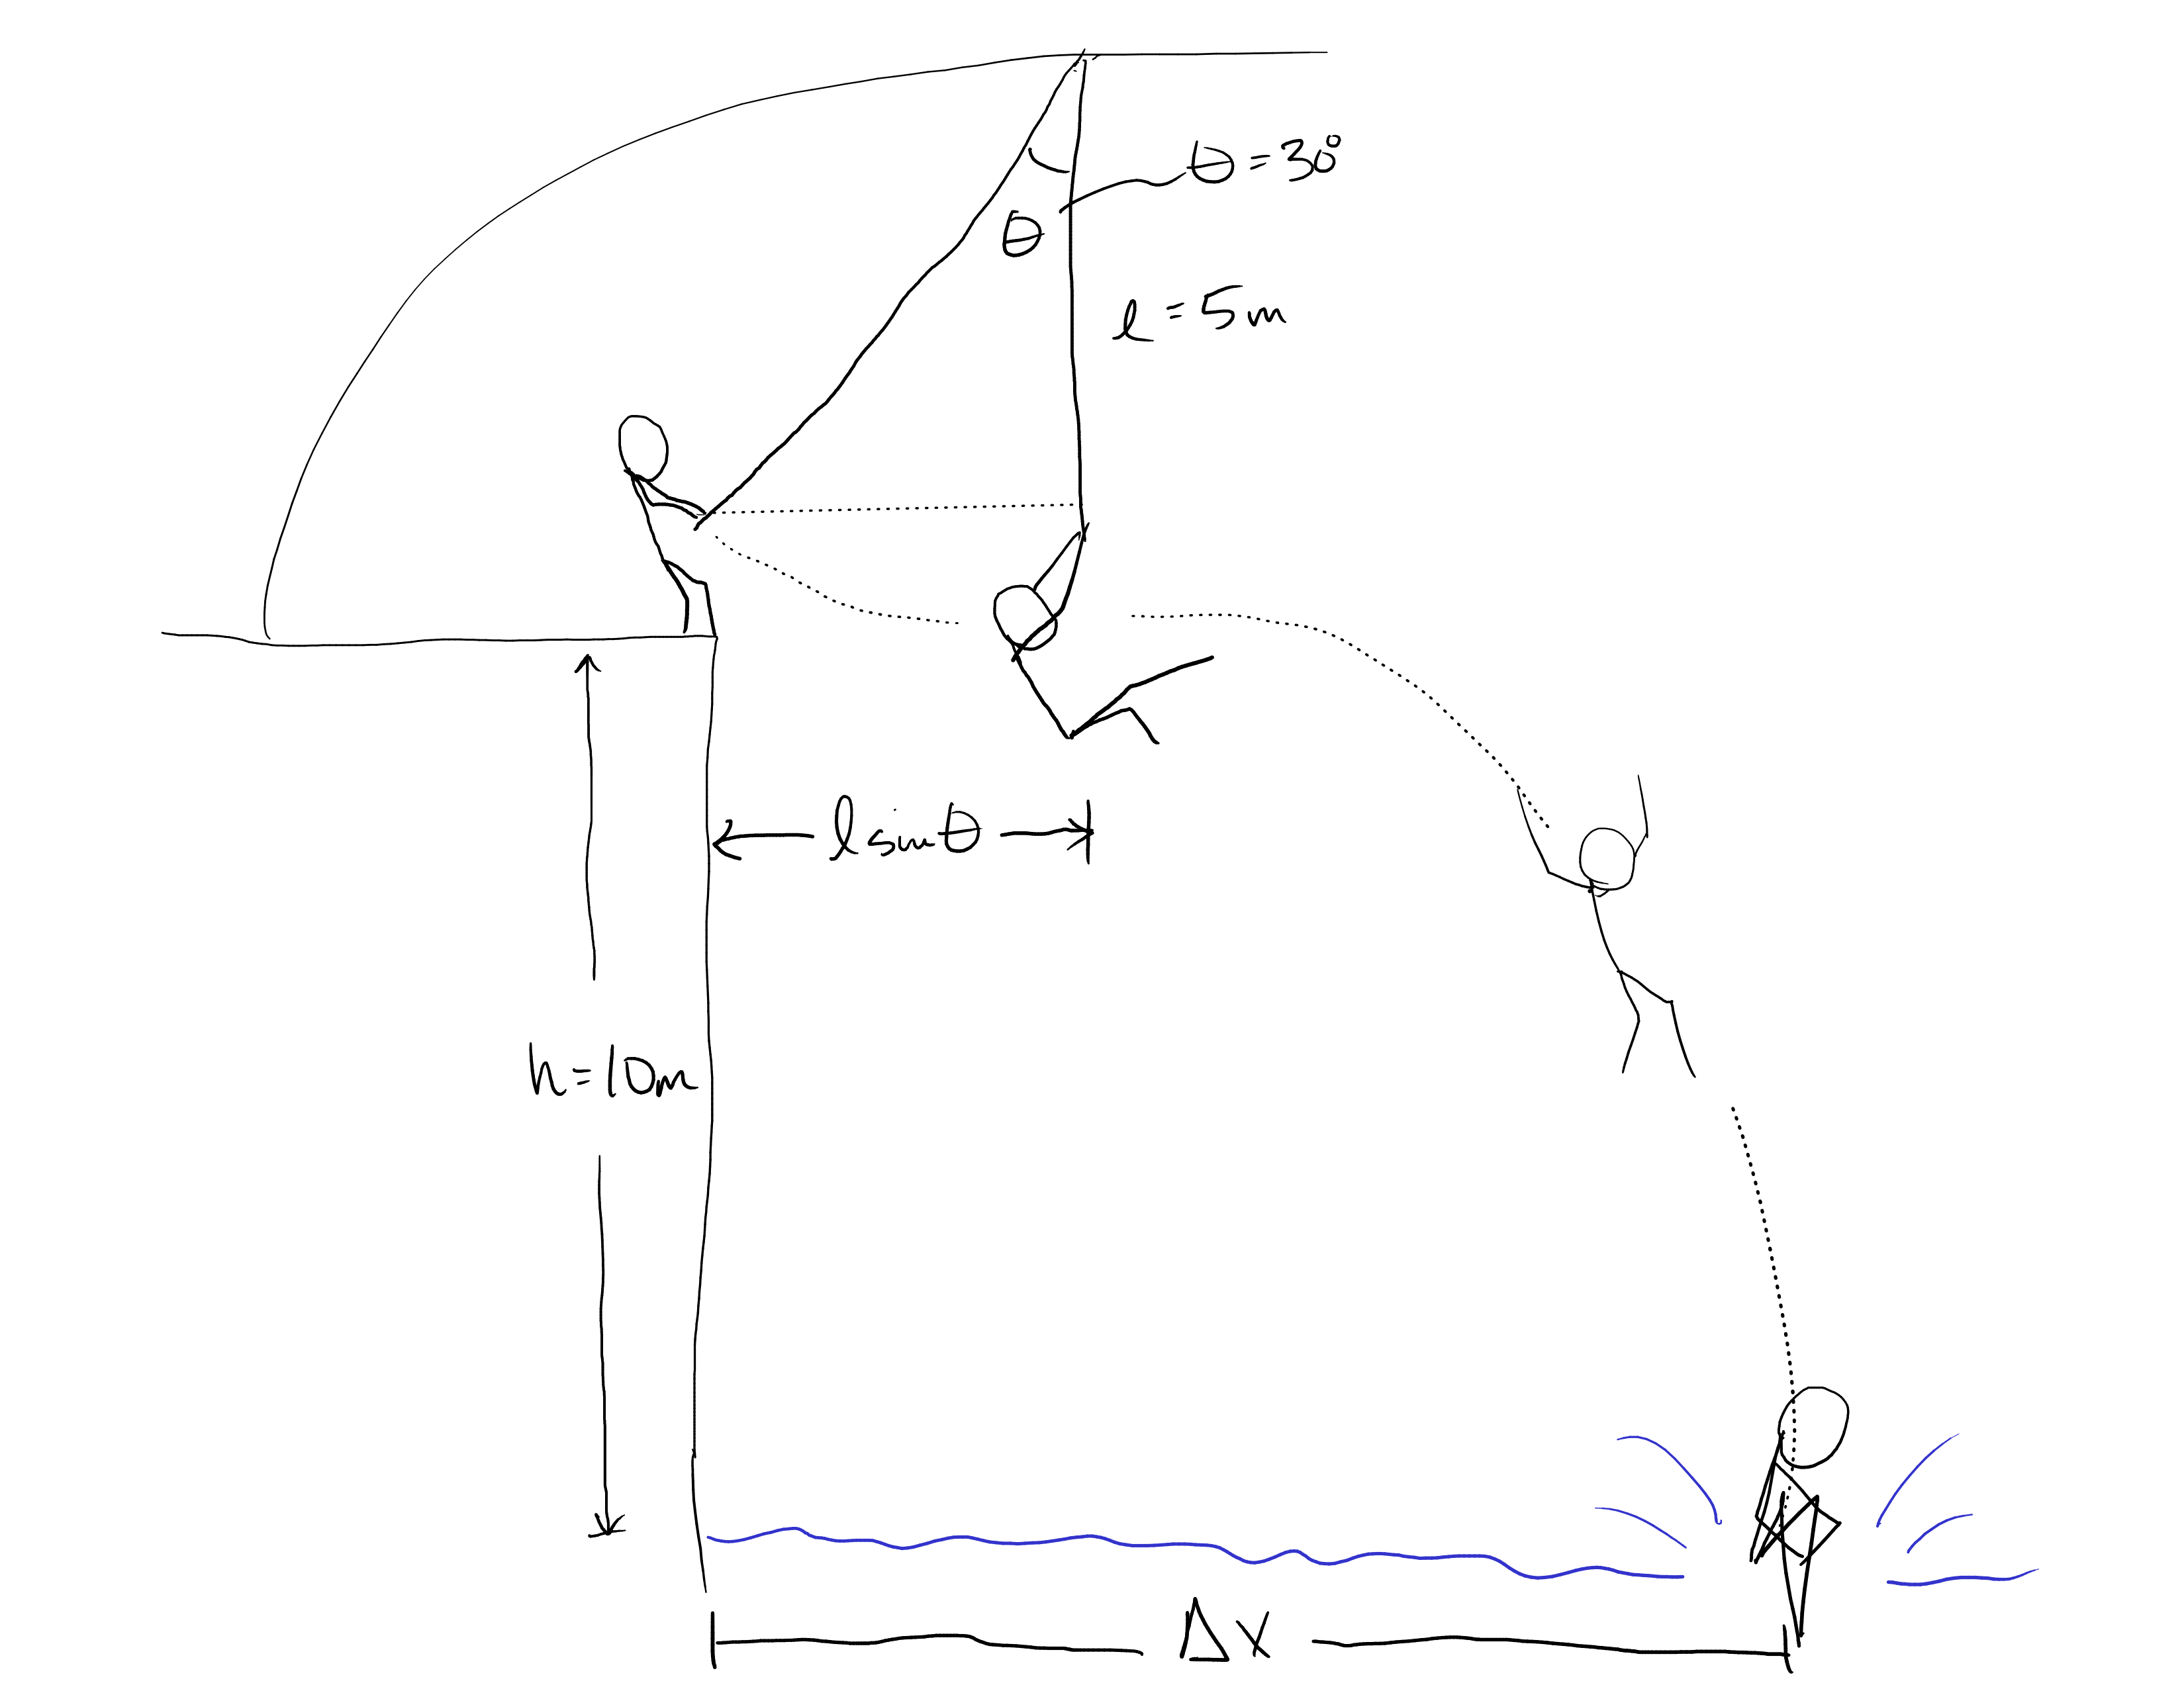
\includegraphics[scale=0.1]{week7-rope-swing.png}



\end{enumerate}